\documentclass{Configuration_Files/PoliMi3i_thesis}

%------------------------------------------------------------------------------
%	REQUIRED PACKAGES AND  CONFIGURATIONS
%------------------------------------------------------------------------------

% CONFIGURATIONS
\usepackage{parskip} % For paragraph layout
\usepackage{setspace} % For using single or double spacing
\usepackage{emptypage} % To insert empty pages
\usepackage{multicol} % To write in multiple columns (executive summary)
\setlength\columnsep{15pt} % Column separation in executive summary
\setlength\parindent{0pt} % Indentation
\raggedbottom  

% PACKAGES FOR TITLES
\usepackage{titlesec}
% \titlespacing{\section}{left spacing}{before spacing}{after spacing}
\titlespacing{\section}{0pt}{3.3ex}{2ex}
\titlespacing{\subsection}{0pt}{3.3ex}{1.65ex}
\titlespacing{\subsubsection}{0pt}{3.3ex}{1ex}
\usepackage{color}

% PACKAGES FOR LANGUAGE AND FONT
\usepackage[utf8]{inputenc} % UTF8 encoding
\usepackage[T1]{fontenc} % Font encoding
\usepackage[11pt]{moresize} % Big fonts
\usepackage{pythonhighlight}

% PACKAGES FOR IMAGES
\usepackage{graphicx}
\usepackage{transparent} % Enables transparent images
\usepackage{eso-pic} % For the background picture on the title page
\usepackage{subfig} % Numbered and caption subfigures using \subfloat.
\usepackage{tikz} % A package for high-quality hand-made figures.
\usetikzlibrary{}
\graphicspath{{./Images/}} % Directory of the images
\usepackage{caption} % Coloured captions
\usepackage{xcolor} % Coloured captions
\usepackage{amsthm,thmtools,xcolor} % Coloured "Theorem"
\usepackage{float}

% STANDARD MATH PACKAGES
\usepackage{amsmath}
\usepackage{amsthm}
\usepackage{amssymb}
\usepackage{amsfonts}
\usepackage{bm}
\usepackage[overload]{empheq} % For braced-style systems of equations.
\usepackage{fix-cm} % To override original LaTeX restrictions on sizes

% PACKAGES FOR TABLES
\usepackage{tabularx}
\usepackage{longtable} % Tables that can span several pages
\usepackage{colortbl}

% PACKAGES FOR ALGORITHMS (PSEUDO-CODE)
\usepackage{algorithm}
\usepackage{algorithmic}

% PACKAGES FOR REFERENCES & BIBLIOGRAPHY
\usepackage[colorlinks=true,linkcolor=black,anchorcolor=black,citecolor=black,filecolor=black,menucolor=black,runcolor=black,urlcolor=black]{hyperref} % Adds clickable links at references
\usepackage{cleveref}
\usepackage[square, numbers, sort&compress]{natbib} % Square brackets, citing references with numbers, citations sorted by appearance in the text and compressed
\bibliographystyle{abbrvnat} % You may use a different style adapted to your field

% OTHER PACKAGES
\usepackage{pdfpages} % To include a pdf file
\usepackage{afterpage}
\usepackage{lipsum} % DUMMY PACKAGE
\usepackage{fancyhdr} % For the headers
\fancyhf{}

% Input of configuration file. Do not change config.tex file unless you really know what you are doing. 
% Define blue color typical of polimi
\definecolor{bluepoli}{cmyk}{0.4,0.1,0,0.4}

% Custom theorem environments
\declaretheoremstyle[
  headfont=\color{bluepoli}\normalfont\bfseries,
  bodyfont=\color{black}\normalfont\itshape,
]{colored}

% Set-up caption colors
\captionsetup[figure]{labelfont={color=bluepoli}} % Set colour of the captions
\captionsetup[table]{labelfont={color=bluepoli}} % Set colour of the captions
\captionsetup[algorithm]{labelfont={color=bluepoli}} % Set colour of the captions

\theoremstyle{colored}
\newtheorem{theorem}{Theorem}[chapter]
\newtheorem{proposition}{Proposition}[chapter]

% Enhances the features of the standard "table" and "tabular" environments.
\newcommand\T{\rule{0pt}{2.6ex}}
\newcommand\B{\rule[-1.2ex]{0pt}{0pt}}

% Pseudo-code algorithm descriptions.
\newcounter{algsubstate}
\renewcommand{\thealgsubstate}{\alph{algsubstate}}
\newenvironment{algsubstates}
  {\setcounter{algsubstate}{0}%
   \renewcommand{\STATE}{%
     \stepcounter{algsubstate}%
     \Statex {\small\thealgsubstate:}\space}}
  {}

% New font size
\newcommand\numfontsize{\@setfontsize\Huge{200}{60}}

% Title format: chapter
\titleformat{\chapter}[hang]{
\fontsize{50}{20}\selectfont\bfseries\filright}{\textcolor{bluepoli} \thechapter\hsp\hspace{2mm}\textcolor{bluepoli}{|   }\hsp}{0pt}{\huge\bfseries \textcolor{bluepoli}
}

% Title format: section
\titleformat{\section}
{\color{bluepoli}\normalfont\Large\bfseries}
{\color{bluepoli}\thesection.}{1em}{}

% Title format: subsection
\titleformat{\subsection}
{\color{bluepoli}\normalfont\large\bfseries}
{\color{bluepoli}\thesubsection.}{1em}{}

% Title format: subsubsection
\titleformat{\subsubsection}
{\color{bluepoli}\normalfont\large\bfseries}
{\color{bluepoli}\thesubsubsection.}{1em}{}

% Shortening for setting no horizontal-spacing
\newcommand{\hsp}{\hspace{0pt}}

\makeatletter
% Renewcommand: cleardoublepage including the background pic
\renewcommand*\cleardoublepage{%
  \clearpage\if@twoside\ifodd\c@page\else
  \null
  \AddToShipoutPicture*{\BackgroundPic}
  \thispagestyle{empty}%
  \newpage
  \if@twocolumn\hbox{}\newpage\fi\fi\fi}
\makeatother

%For correctly numbering algorithms
\numberwithin{algorithm}{chapter}

%----------------------------------------------------------------------------
%	NEW COMMANDS DEFINED
%----------------------------------------------------------------------------

% EXAMPLES OF NEW COMMANDS
\newcommand{\bea}{\begin{eqnarray}} % Shortcut for equation arrays
\newcommand{\eea}{\end{eqnarray}}
\newcommand{\e}[1]{\times 10^{#1}}  % Powers of 10 notation

%----------------------------------------------------------------------------
%	ADD YOUR PACKAGES (be careful of package interaction)
%----------------------------------------------------------------------------
\definecolor{codegreen}{rgb}{0,0.6,0}
\definecolor{codegray}{rgb}{0.5,0.5,0.5}
\definecolor{codepurple}{rgb}{0.58,0,0.82}
\definecolor{backcolour}{rgb}{0.95,0.95,0.92}
\usepackage{color}   %May be necessary if you want to color links
\usepackage{hyperref}
\usepackage{graphicx}
\usepackage[utf8]{inputenc}
\usepackage{listings}
\usepackage{xcolor}
\hypersetup{
colorlinks=true, %set true if you want colored links
linktoc=all,     %set to all if you want both sections and subsections linked
linkcolor=black,  %choose some color if you want links to stand out
urlcolor=blue,
}
\lstdefinestyle{mystyle}{
backgroundcolor=\color{backcolour},
commentstyle=\color{codegreen},
keywordstyle=\color{magenta},
numberstyle=\tiny\color{codegray},
stringstyle=\color{codepurple},
basicstyle=\ttfamily\footnotesize,
breakatwhitespace=false,
breaklines=true,
captionpos=b,
keepspaces=true,
numbers=left,
numbersep=5pt,
showspaces=false,
showstringspaces=false,
showtabs=false,
tabsize=2
}

\lstset{style=mystyle}


%----------------------------------------------------------------------------
%	ADD YOUR DEFINITIONS AND COMMANDS (be careful of existing commands)
%----------------------------------------------------------------------------

%----------------------------------------------------------------------------
%	BEGIN OF YOUR DOCUMENT
%----------------------------------------------------------------------------

\begin{document}

\fancypagestyle{plain}{%
\fancyhf{} % Clear all header and footer fields
\fancyhead[RO,RE]{\thepage} %RO=right odd, RE=right even
\renewcommand{\headrulewidth}{0pt}
\renewcommand{\footrulewidth}{0pt}}

%----------------------------------------------------------------------------
%	TITLE PAGE
%----------------------------------------------------------------------------

\pagestyle{empty} % No page numbers
\frontmatter % Use roman page numbering style (i, ii, iii, iv...) for the preamble pages

\puttitle{
title=SMBUD Project - Spark,
name1=Gabriele Ginestroni, % Author Name and Surname
name2=Giacomo Gumiero,
name3=Lorenzo Iovine,
name4=Nicola Landini,
name5=Francesco Leone,
academicyear=2022-2023,
groupnumber=10
} % These info will be put into your Title page


%----------------------------------------------------------------------------
%	PREAMBLE PAGES: ABSTRACT (inglese e italiano), EXECUTIVE SUMMARY
%----------------------------------------------------------------------------
\startpreamble
\setcounter{page}{1} % Set page counter to 1

%----------------------------------------------------------------------------
%	LIST OF CONTENTS/FIGURES/TABLES/SYMBOLS
%----------------------------------------------------------------------------

% TABLE OF CONTENTS
\thispagestyle{empty}
\tableofcontents % Table of contents 
\thispagestyle{empty}
\cleardoublepage

%-------------------------------------------------------------------------
%	THESIS MAIN TEXT
%-------------------------------------------------------------------------
% In the main text of your thesis you can write the chapters in two different ways:
%
%(1) As presented in this template you can write:
%    \chapter{Title of the chapter}
%    *body of the chapter*
%
%(2) You can write your chapter in a separated .tex file and then include it in the main file with the following command:
%    \chapter{Title of the chapter}
%    \input{chapter_file.tex}
%
% Especially for long thesis, we recommend you the second option.

\addtocontents{toc}{\vspace{2em}} % Add a gap in the Contents, for aesthetics
\mainmatter % Begin numeric (1,2,3...) page numbering

\chapter{Introduction}
\label{ch:introduction}
In this chapter will be presented the problem specification and the hypothesis under which the database is implemented.


\chapter{Data Structure}
\label{ch:data_struct}
In this chapter will be described the dataframes used. We created the following dataframes using the same JSONs of the MONGO DB part of the project but differently from MONGO DB we created a third dataframe for the \emph{venue} moving some of the attributes.
\section{Article structure}
In the following image we can see the schema of  \emph{Article}.\newline
Note: unlike the previous implementation we moved the fields: \emph{issue}, \emph{volume}, \emph{publisher}, \emph{venue\_raw} inside the article.\newline
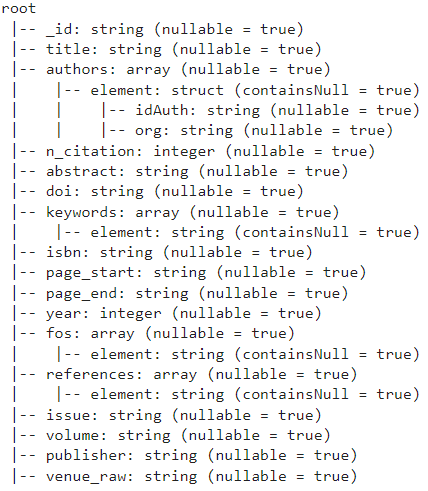
\includegraphics{article_schema}

\section{Author structure}
In the following image we can see the schema of \emph{Author}.\newline
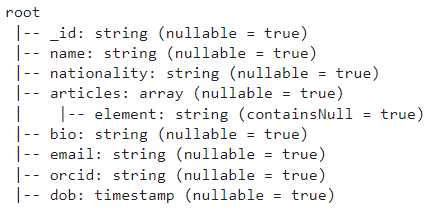
\includegraphics{author_schema}

\section{Venue structure}
In the following image we can see the schema of \emph{Venue}.\newline
Note: unlike previous implementation we added the \emph{city} field that is randomly populated.
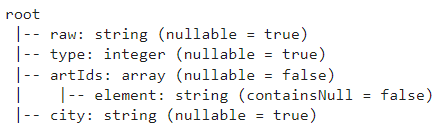
\includegraphics{venue_schema}

\chapter{Data Import}
\label{ch:data_import}
\section{Setup}
\begin{python}
from pyspark.sql import SparkSession
from pyspark.sql.types import StructType, StructField, IntegerType, StringType, ArrayType
from pyspark.sql.functions import col, to_timestamp, rand, lit, collect_list, array

spark = SparkSession.builder \
    .master("local") \
    .appName("SparkByExamples.com") \
    .getOrCreate()
\end{python}

\section{Article Custom Schema}
\begin{python}
schemaArticle = StructType([
    StructField('_id', StringType(), True),
    StructField('title', StringType(), True),
    StructField('authors',
        ArrayType(
        StructType([
            StructField('idAuth', StringType(), True),
            StructField('org', StringType(), True)
        ]), True)
    ),
    StructField('n_citation', IntegerType(), True),
    StructField('abstract', StringType(), True),
    StructField('doi', StringType(), True),
    StructField('keywords', ArrayType(StringType()), True),
    StructField('isbn', StringType(), True),
    StructField('page_start', StringType(), True),
    StructField('page_end', StringType(), True),
    StructField('year', IntegerType(), True),
    StructField('fos', ArrayType(StringType()), True),
    StructField('references', ArrayType(StringType()), True),
    StructField('venue',
        StructType([
            StructField('raw', StringType(), True),
            StructField('type', IntegerType(), True),
            StructField('issue', StringType(), True),
            StructField('volume', StringType(), True),
            StructField('publisher', StringType(), True)
        ])
    ),
])
\end{python}
\bigskip
We decided to use import from schema to explicitly show data structure:
\begin{python}
df_articles = spark.read.schema(schemaArticle).json("../dblp_sample_filtered_spark.json", multiLine=True)
\end{python}
\bigskip
The attributes \verb |issue|, \verb |volume| and \verb |publisher| inside venue are moved back in the root structure
and removed from the inner struct:
\begin{python}
df_articles = df_articles.withColumn("issue", col("venue.issue")) \
                        .withColumn("volume", col("venue.volume")) \
                        .withColumn("publisher", col("venue.publisher")) \
                        .withColumn("venue", col("venue").dropFields("issue", "volume", "publisher"))
\end{python}

\section{Venue Collection Structure}
A new dataframe is created with attributes of venue and the \verb |_id| of the article, then it is all grouped by
venue attributes and, for each venue, a list of the articles ids is created. Finally we drop rows with null \verb|raw|
to delete inconsistent tuple.
\begin{python}
df_venues = df_articles.select("venue.raw", "venue.type", "_id") \
                        .groupBy("raw", "type") \
                        .agg(collect_list("_id").alias("artIds")) \
                        .dropna(subset=["raw"])
\end{python}
\bigskip
Now we can keep only the raw attribute of the venue:
\begin{python}
df_articles = df_articles.withColumn("venue_raw", col("venue.raw")).drop("venue")
\end{python}
\bigskip
In the end, we add a generated field inside venues collection: for each venue a random city is selected that should
represent the place where the venue was held.
\begin{python}
citiesList = ["New York", "London", "Paris", "Berlin", "Madrid", "Rome", "Dublin", "Copenhagen", "Vienna", "Amsterdam", "Brussels", "Lisbon", "Prague", "Athens", "Budapest", "Warsaw", "Zurich", "Luxembourg", "Oslo", "Stockholm", "Helsinki", "Moscow", "Istanbul", "Kiev", "Minsk", "Belgrade", "Bucharest", "Sofia", "Tallinn", "Riga", "Vilnius", "Tbilisi", "Yerevan", "Baku", "Dubai", "Abu Dhabi", "Doha", "Manama", "Muscat", "Riyadh", "Jeddah", "Mecca", "Medina", "Kuala Lumpur", "Singapore", "Hong Kong", "Shanghai", "Beijing", "Tokyo", "Seoul", "Bangkok", "Manila"]
cities = array([lit(city) for city in citiesList])
df_venues = df_venues.withColumn("city", cities.getItem((rand() * len(citiesList)).cast("int")))
\end{python}

\section{Author Collection Structure}
In order to handle authors' collection, we simply import from json with autogenerated schema, applying a conversion from
string to timestamp.
\begin{python}
df_authors = spark.read.json("../dblp_sample_reverted_filtered_spark.json", multiLine=True)
df_authors = df_authors.withColumn("dateofbirth", to_timestamp(df_authors["dob"], "yyyy-MM-dd'T'HH:mm:ss'Z'")) \
                        .drop("dob") \
                        .withColumnRenamed("dateofbirth", "dob")
\end{python}


\end{document}
